\textbf{COLUNI 2025 -- Questão 38}\par\medskip Observe as imagens abaixo, relativas ao processo de divisão dos territórios palestinos e israelenses:

\begin{center}
\begin{minipage}[t]{0.49\linewidth}\centering
Mapa 01 – 1948\\
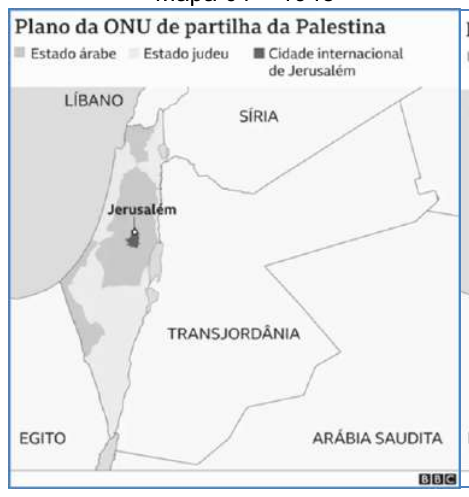
\includegraphics[width=\linewidth]{static/simulados/coluni/figuras/2025/questao-38/figura-1.png}
\end{minipage}\hfill\begin{minipage}[t]{0.49\linewidth}\centering
Mapa 02 - 2021\\
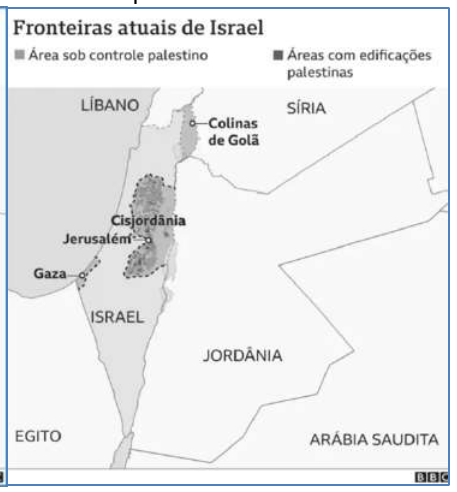
\includegraphics[width=\linewidth]{static/simulados/coluni/figuras/2025/questao-38/figura-2.png}
\end{minipage}
\end{center}

\noindent BBC NEWS BRASIL. Como território palestino encolheu e Israel cresceu desde partilha da ONU em 1948. \textbf{BBC News Brasil}, 18 maio 2021. Disponível em: https://www.bbc.com/portuguese/internacional-57147042. Acesso em: 8 ago. 2024.

\par

O chamado conflito árabe-israelense tem origem no processo de expansão imperialista do século XIX, que atingiu a região da Palestina, com disputas territoriais entre turco-otomanos, franceses e britânicos, com “desfecho” na primeira metade do século XX. Desde a Primeira Guerra Mundial, com intensificação, após a Segunda Guerra, finalizada em 1945, uma nova disputa surgiu. Judeus sionistas, buscavam a constituição de um Estado após o genocídio capitaneado pelo nazi-fascismo. De outro lado, a população Palestina, tentava se livrar da dominação colonial dos Britânicos. A, então recém-criada, Organização das Nações Unidas (ONU) tentou conciliar a disputa em jogo formulando, em 1948, um plano de divisão territorial que contemplaria a solução de dois Estados: Israel e Palestina. Entretanto, ao longo dos anos, uma sucessão de guerras territoriais desmobilizou a proposta da ONU, levando a uma ampliação das áreas sob o controle do Estado de Israel, configurando o que é considerado, especialmente pelos palestinos, uma guerra de ocupação colonial. Em outubro de 2023, os ataques terroristas cometidos pelo grupo palestino Hamas, contra militares e civis israelenses, colocaram o conflito árabe-israelense, novamente, nos holofotes mundiais. Desde então, a resposta israelense já foi classificada pela Agência da ONU de Assistência aos Refugiados Palestinos (Unrwa) como uma “destruição apocalíptica”, marcada pelo deslocamento forçado da população palestina por um território devastado por bombardeios, com saldo de dezenas de milhares de mortos.

A partir das imagens e de seus conhecimentos sobre o conflito entre palestinos e israelenses, é CORRETO afirmar:
\begin{enumerate}
\item As fronteiras atuais entre Israel e Palestina estão claramente definidas e reconhecidas internacionalmente, com a Cisjordânia e Gaza sendo parte integrante do Estado Palestino independente, desde 1993.
\item As fronteiras atuais foram estabelecidas, após a Guerra do Yom Kippur, em 1973, resultando em dois Estados reconhecidos, com a Palestina controlando Jerusalém Oriental e Israel controlando a Cisjordânia e Gaza.
\item A Faixa de Gaza está sob o controle total da Autoridade Palestina, que mantém boas relações com Israel, o que facilita o fluxo de bens e de pessoas, através das fronteiras entre os dois países, minimizando os impactos da recente guerra.
\item A Faixa de Gaza, desde 2007, é controlada pelo Hamas e está completamente isolada por barreiras israelenses, sem qualquer conexão terrestre com a Cisjordânia, resultando em um bloqueio humanitário severo.
\end{enumerate}
